\graphicspath{{content/2_design/figures/}}
\section{Range sensor}
\subsection{Sensor power \& output}{\label{rangeSensor_powerOutput}}
The range sensor requires \SI{5}{V_{dc}} power and will draw around \SI{15}{mA}. Since the LD1117V provides a stable 5.0 V output and is capable
of providing up to 800 mA of current, the sensor will be powered directly from this regulator.

The sensor's echo output is a PWM wave of varying duty cycle $\tau$ and $f_{PWM} = \SI{16}{Hz}$.
This signal's amplitude could be as high as 5 V (TTL level). The maximum output $A_{max}$ \textit{after} unity filtering,
however, will be determined by the maximum duty cycle, $t_{max}$. Since a distance of $D_{max} = \SI{1}{m}$ and $D_{min} = \SI{5}{cm}$,
Equations \ref{eqn:sensor_distanceFormula} and \ref{eqn:pwm_filtered_amplitude} can be used to calculate:
\begin{itemize}
  \item At $D_{max}$, $t_{max} \approx \SI{5.9}{ms}$, $\tau_{max} = \frac{\SI{5.9}{ms}}{1/16} \approx 9.5 \%$ and $A_{max} = (\SI{5}{V}) \cdot (9.5 \%) = \SI{475}{mV} $.
  \item At $D_{min}$, $t_{min} \approx \SI{0.29}{ms}$, $\tau_{min} = \frac{\SI{0.29}{ms}}{1/16} \approx 0.47 \%$ and $A_{min} = (\SI{5}{V}) \cdot (0.47 \%) = \SI{23}{mV} $.
\end{itemize}

\subsection{Filter selection}{\label{rangeSensor_filterSelection}}

To determine the filter's order, rise time and noise requirements should be considered:
\begin{itemize}
  \item After filtering, since gain $\approx \frac{\SI{3}{V}}{\SI{475}{mV}} \approx \SI{7}{V/V}$, filter ripple must be under $ \frac{\SI{70}{mV}}{7} = \SI{7}{mV}$.
  \item A 10\% to 90\% rise time ($t_r$) of \SI{1.5}{s} should be adhered to.
\end{itemize}

\noindent These specifications result in the requirement that $A_{dB}$ at $f_{PWM} = 20 \log \left[ \frac{\SI{5}{V}}{\SI{7}{mV}} \right] \approx \SI{60}{dB}$.
A \nth{3} order filter with $f_c = \SI{1}{Hz}$ will be used, as a \nth{2} order may be tolerance-sensitive.
This provides $t_r \approx 0.63 s$ and $A_{dB} \approx 72 dB $ [\ref{filter_formulae}].

\begin{table}[!h]
  \centering
  \renewcommand{\arraystretch}{1.2}
  \begin{tabular}{ |c|c|p{2.5cm}|p{2.5cm}|p{3.5cm}| }
    \hline
    \textbf{Filter type}  & \textbf{Design Spec.}         & \textbf{Cutoff $f_c$}     & \textbf{Rise time $t_r$}        & \textbf{Attenuation $A_{dB}$}       \\
    \hline
    \nth{1} order            & Rise Time                     & 0.233 Hz                  & 1.5 s                           & 37 dB                               \\
                             & Attenuation                   & 0.016 Hz                  & 22 s                            & 60 dB                               \\ \hline
    \nth{2} order            & Rise Time                     & 0.350 Hz                  & 1.5 s                           & 66 dB                               \\
                             & Attenuation                   & 0.505 Hz                  & 1.038 s                         & 60 dB                               \\ \hline
    \nth{3} order (cascade)  & Rise Time                     & 0.420 Hz                  & 1.5 s                           & 95 dB                               \\
                             & Attenuation                   & 1.600 Hz                  & 0.394 s                         & 60 dB                               \\ \hline
  \end{tabular}
  \caption{Filter type vs Rise Time and Attenuation using [\ref{filter_formulae}]}
  \label{tab:range_sensor_filter_comparison}
\end{table}

\subsection{Configuration}\label{rangeSensor_circuitConfig}

A "two-and-a-half" stage configuration will be used. The first stage is a gain/offset and \nth{1} order filter,
and is placed first in order to amplify the signal above the MCP's 35 mV floor. The second stage is unity-gain \nth{2} order filter.
A non-inverting amplifier will be used for stage 1, and a Sallen-Key topology for stage 2. Since the quiescent current for each op-amp is
$\SI{70}{uA}$ \cite{datasheetMCP6242}, stage 1 \& 2 will be allocated $\SI{400}{\micro\ampere}$ and $\SI{200}{\micro\ampere}$ respectively.

\begin{figure}[!htb]
  \centering
  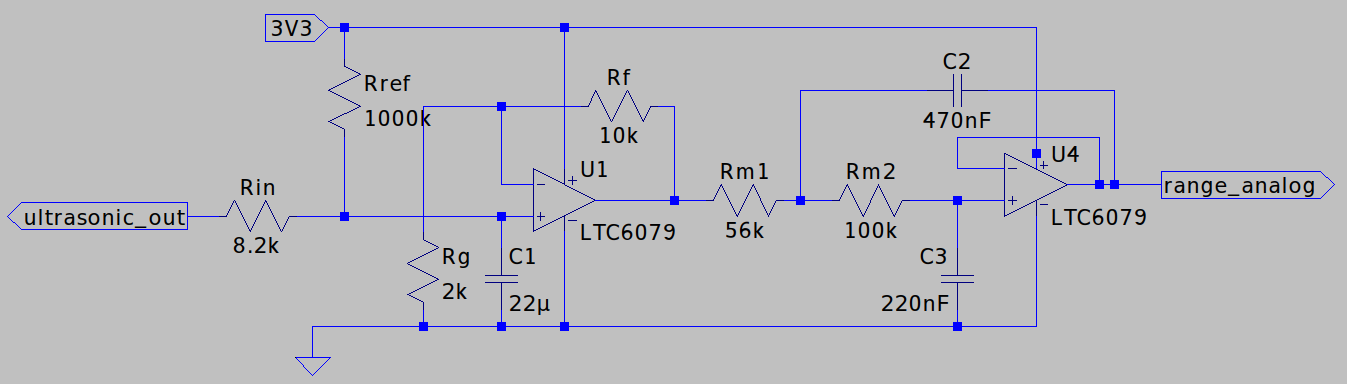
\includegraphics[width=0.8\textwidth]{rangeSensor_circuitDiagram}
  \caption{Final range sensor amplifier circuit diagram}
  \label{fig:rangeSensor_circuitDiagram}
\end{figure}

\subsection{Gain stage}

This stage will be powered by the 3.3 V regulator. As this is a low-gain circuit, input bias voltages can be neglected.
Slew rate and CMMR imbalance can also be ignored due to the low-frequency, single-ended use of the op-amp.
Voltage rail saturation does not need to be considered at the circuit output, as $\SI{0.3}{V} < V_{out} < \SI{3}{V}$,
and has already been catered for at the input, as discussed in Section \ref{rangeSensor_circuitConfig}.
Using the equations at \cite{gainOffset30Seconds}, and the expected input ranges from the filter stage,
gain $m = \frac{\SI{3}{V} - \SI{0.3}{V}}{\SI{475}{mV} - \SI{23}{mV}} = \SI{5.97}{\volt\per\volt}$,
and offset $b = \SI{0.3}{V} - m \times \SI{23}{mV} \approx \SI{163}{mV}$:

\begin{itemize}
  \item With idle current $I_Q = \frac{V_{out}}{R_f + R_g}$, and $V_{out(max)} = \SI{3.3}{V}$, $(R_f + R_g)_{min} = \frac{\SI{3.3}{V}}{\SI{400}{\micro\ampere}} = \SI{8.25}{\kilo\ohm}$.
  \item Since the offset voltage is low (i.e. $R_{ref}$ will be high), first choose $R_{ref} = \SI{820}{\kilo\ohm} + \SI{470}{\kilo\ohm} \textnormal{pot} \approx \SI{1000}{\kilo\ohm}$.
        A potentiometer is used to tune the offset.
  \item Calculate $R_{in} = \frac{R_{ref} \times b}{V_{ref} \times m} \approx \SI{8.2}{\kilo\ohm}$ with $V_{ref} = \SI{5}{V}$ and $C_1 = \frac{1}{2 \pi f_c R_1} \approx \SI{22}{\micro\farad}$.
  \item Choose $R_f = \SI{10}{\kilo\ohm}$ to satisfy the current requirements.
  \item Calculate $R_g = \frac{R_{ref} \times R_f}{m \times (R_{in} + R_{ref}) - R_{ref}} \approx \SI{2}{\kilo\ohm}$. To tune the gain, choose $R_g = \SI{1.5}{k} + \SI{1}{\kilo\ohm}\textnormal{pot}$.
\end{itemize}


\subsection{Filter stage}{\label{rangeSensor_filterDesign}}

This stage will use the 3.3 V regulator to clip the circuit output for use with the MCU.
This results in the \nth{2} order stage transfer function $H(s) = \frac{1}{1 + 0.2251 s + 0.02533 s^2} = \frac{1}{1 + a_1 s + b_1 s^2}$ with $\zeta = 0.707$. Now, component values can be chosen.
Formulae from \cite{filterDesign} will be used:

\begin{itemize}
  \item Since both capacitors are open-circuit during DC, the idle current is very low. A maximum step input will result in a surge of current through $C_2$ to ground.
        With $V_{in(max)} = \SI{5}{V}$, $(R_{m1} + R_{m2})_{min} = \frac{\SI{5}{V}}{\SI{200}{\micro\ampere}} = \SI{25}{\kilo\ohm}$.
  \item Since $C_3 = \frac{a_1}{2 \pi f_c (R_{m1} + R_{m2})}$ \cite{filterDesign}, choose $C_3 = \SI{220}{nF}$ so that $R_{m1} + R_{m2} \approx \SI{160}{\kilo\ohm}$.
  \item To meet $C_2 \geq C_3 \cdot \frac{4 \cdot b_1}{a_1 ^2} \approx 2 C_3 $ \cite{filterDesign}, choose $C_2 = \SI{470}{nF}$.
  \item Since $C_3 \cdot C_2 = \frac{b_1}{((2 \pi f_c)^2 R_{m1} R_{m2})}$, and $R_{m1} + R_{m2} = \SI{450}{\kilo\ohm}$, solve to obtain $R_{m1} = \SI{61}{\kilo\ohm}$ and $R_{m2} = \SI{99}{\kilo\ohm}$.
        Choose $R_{m1} = \SI{56}{\kilo\ohm}$ and $R_{m2} = \SI{100}{\kilo\ohm}$ as practical values.
\end{itemize}